%\IEEEraisesectionheading{\section{Introduction} \label{chp:understanding_understandability}}
\section*{Introduction} 
\label{chp:understanding_understandability}

%\IEEEPARstart{S}{earch}
Search engines are concerned with retrieving relevant information to support a user's information seeking task. Commonly, signals about the topicality or aboutness of a piece of information with respect to a query are used to estimate relevance, with other relevance dimensions like understandability, trustworthiness, etc.~\cite{zhang2014multidimensional} being relegated to a secondary position, or completely neglected. While this may be a minor problem for many information seeking tasks, there are some specific tasks in which dimensions other than topicality have an important role in the information seeking and decision making process. The seeking of health information and advice on the Web by the general public is one such task. 

A key problem when searching the Web for health information is that this can be too technical, unreliable, generally misleading, and can lead to unfounded escalations and poor decisions~\cite{white09b}. Where correct information exists, it can be hard to find and digest amongst the noise, spam, technicalities, and irrelevant information. In \textit{high-stakes search tasks} such as this, access to poor information can lead to poor decisions which ultimately can have a significant impact on our health and well-being~\cite{white09b,white13}. In this work we are specifically interested in the understandability of health information retrieved by search engines, and in improving search results to favour information understandable by the general public. We leave addressing reliability and trustworthiness of the retrieved information to future work; however this can be achieved by extending the framework we investigate here.

The use of general purpose Web search engines like Google, Bing and Baidu for seeking health advice has been largely analysed, questioned and criticised~\cite{graber99,fitzsimmons10,wiener13,patel13,atcherson14,meillier17,ellimoottil12}, despite the commendable efforts these services have put into providing increasingly better health information, e.g., the Google Health Cards~\cite{gabrilovich2016cura}. 

Ad-hoc solutions to support the general public in searching and accessing health information on the Web have been implemented, typically supported by government initiatives or medical practitioner associations, e.g., \url{HealthOnNet.org} (HON) and \url{HealthDirect.gov.au}, among others. These solutions aim to provide \textit{better} health information to the general public. For example, HON's mission statement is ``to guide Internet users to reliable, understandable, accessible and trustworthy sources of medical and health information''. But, do the solutions these services currently employ actually provide this type of information to the health-seeking general public? As an illustrative example, we analysed the top 10 search results retrieved by HON\footnote{Results retrieved on 01/10/2017.} in answer to 300 search queries from CLEF 2016 eHealth \todo{(see Section~\ref{sec:data})}. Figure~\ref{fig:dist} reports the cumulative distribution of understandability scores for these search results (note, we did not assess their topical relevance here). Understandability scores were computed with the most effective readability formula and settings from \todo{Section~\ref{sec:which_preprocessing}} (Dale-Chall Index), and express how easy is to understand a Web page. Low scores correspond to easy to understand Web pages. We report also the scores for the ``optimal'' search results (Oracle), as found in CLEF 2016 (relevant results that have the highest understandability scores), along with the scores for the best retrieval method from \todo{Section~\ref{sec:results}}. The results clearly indicate that, despite solutions like HON being explicitly aimed at supporting access to understandable health information, they often fail to do so.

%In this article we proposed and investigated methods for the estimation of the understandability of health information in Web pages. In doing so, we also studied the influence of HTML processing methods on these estimations, and their pitfalls. Then, we investigated how understandability estimations can be integrated into retrieval methods to enhance the quality of the retrieved health information, with particular attention to its understandability by the general public. 
%This paper makes a concrete contribution to practice, as it informs health search engines specifically tailored to the general public about the best methods they should adopt. 

In this article we aim to establish methods and best practice for developing search engines that retrieve \textit{relevant and understandable} health advice from the Web. The overall contributions of this article can be \todo{summarized} as:
\begin{enumerate}
\item We propose and investigate methods for the estimation of the understandability of health information in Web pages: a large number of medically-focused features are grouped in meaningful categories and their contribution to the understandability estimation task is carefully measured;
\item We further study the influence of HTML processing methods on these estimations and their pitfalls, extending our previous work that has shown how this often ignored aspect greatly impacts effectiveness~\cite{palotti15};
\item We further investigate how understandability estimations can be integrated into retrieval methods to enhance the quality of the retrieved health information with particular attention to its understandability by the general public. New models are explored in this article, also extending our previous work~\cite{palotti2016ranking};
\end{enumerate}

This paper makes concrete contributions to practice, as it informs health search engines specifically tailored to the general public (for example the HON or HealthDirect services referred to above) about the best methods they should adopt, but they currently don't. These are novel and significant contributions, as no previous work has systematically analysed the influence of the components at play in this study and we show that these greatly influence retrieval effectiveness and thus delivery of relevant and understandable health advice.
%\todo{The famous Reviewer 2 complained about this sentence specifically.}
%\todo{In general we still need here a strong novelty claim}

\begin{figure}[t!]
   \centering
    %\vspace{-0.5cm}
   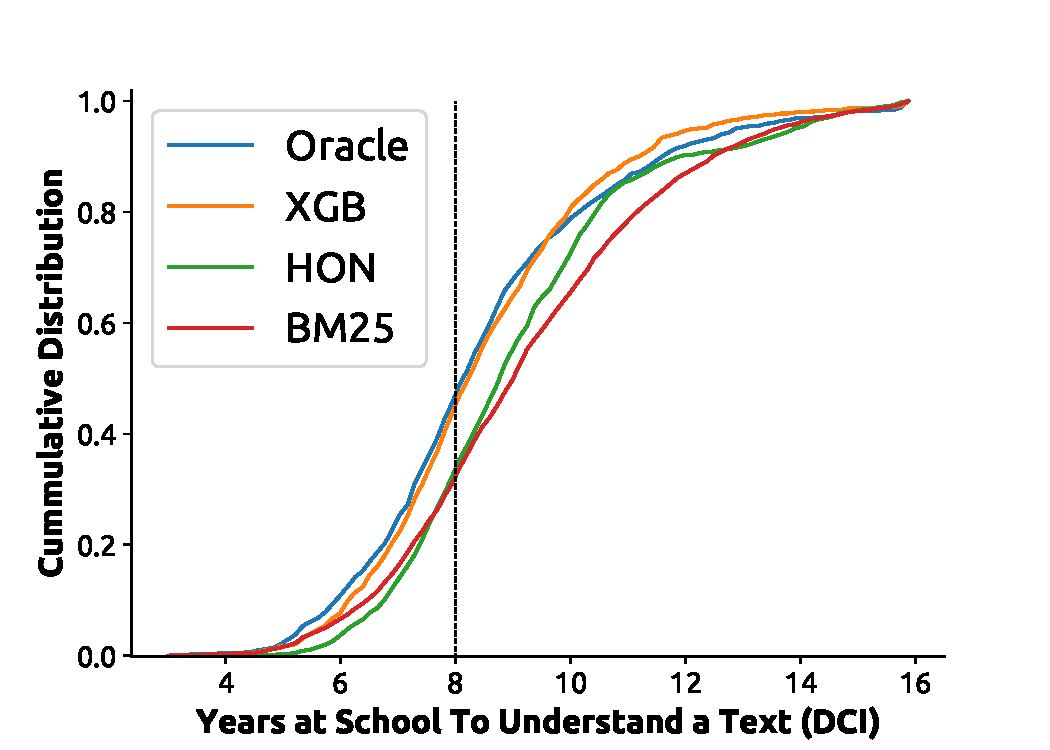
\includegraphics[width=.51\textwidth]{graphics/cumdist}
    %\vspace{-0.2cm}
    \caption{Distribution of Dale-Chall Index (DCI) of search results. DCI measures the years of schooling required to understand a document. The average US resident reads at or below an 8th grade level (dashed line)\cite{cowan04,wallace04,davis04,stossel12}, which is the level suggested by NIH for health information on the Web~\cite{clear94}. The distribution for HON is similar to that of the baseline used in this article (BM25). Our best method (XGB) re-ranks documents to provide more understandable results; its distribution is similar to that of an ``Oracle'' system.}
   \label{fig:dist}
\end{figure}


